\documentclass[a4paper,12pt]{article}

%------------------------------------------------------------------------------------------%
% Déclaration des packages
%------------------------------------------------------------------------------------------%

\usepackage[french]{babel}
\frenchbsetup{StandardLists=true}
\usepackage{enumitem}
\usepackage[T1]{fontenc}
\usepackage{geometry} % pour gérer les dimensions des marges
\usepackage{eso-pic} % pour dessiner la marge
\usepackage{lipsum} % pour générer du contenu texte
\usepackage[cyr]{aeguill} % Police vectorielle TrueType, guillemets fran¸cais
\usepackage{epsfig} % pour g´erer les images
\usepackage{amsmath, amsthm} % tr`es bon mode math´ematique
\usepackage{amsfonts,amssymb}% permet la definition des ensembles
\usepackage{float} % pour le placement des figure
\usepackage{url} 
\usepackage[utf8]{inputenc}
\usepackage{amssymb}
\usepackage{graphicx}
\usepackage{ulem}
\usepackage{array}	
\usepackage{listings}
\usepackage{siunitx}
\usepackage{fancybox}
\usepackage{wrapfig}
\usepackage{caption}
 \usepackage{hyperref}
\usepackage{listings}
\usepackage{xcolor}
\usepackage{booktabs}
\usepackage{fancyhdr}
\usepackage{tabularx}
\usepackage[style=authoryear,backend=biber]{biblatex}
\addbibresource{biblio.bib} 

\lstdefinelanguage{Dockerfile}{
  keywords={FROM, RUN, CMD, LABEL, MAINTAINER, EXPOSE, ENV, ADD, COPY, ENTRYPOINT, VOLUME, USER, WORKDIR, ARG, ONBUILD, STOPSIGNAL, HEALTHCHECK, SHELL},
  keywordstyle=\color{blue}\bfseries,
  identifierstyle=\color{black},
  sensitive=false,
  comment=[l]{\#},
  commentstyle=\color{gray}\ttfamily,
  stringstyle=\color{green},
  morestring=[b]",
  morestring=[b]',
}

\lstdefinelanguage{Python}{
  keywords={True, False, None, await, break, class, def, if, else, elif, for, while, continue, return, and, or, not, in, is, try, except, finally, raise, assert},
  keywordstyle=\color{blue}\bfseries,
  ndkeywords={import, from, as, with, print, yield},
  ndkeywordstyle=\color{darkgray}\bfseries,
  identifierstyle=\color{black},
  comment=[l]{\#},
  commentstyle=\color{green}\ttfamily,
  stringstyle=\color{green},
  morestring=[b]',
  morestring=[b]",
  sensitive=true,
}


\pagestyle{fancy}
\fancyhf{} % Efface les configurations précédentes
\fancyhead[L]{AI referent apprenticeship} % Titre du rapport à gauche
\fancyhead[C]{SAPLABS} % Numéro de page au centre
\fancyhead[R]{HADDOU Amine} % Nom de l'auteur à droite
\fancyfoot[R]{\thepage} % Numéro de page au centre
\fancyfoot[L]{Master 1 informatique\\parcours Intelligence Artificielle} % Numéro de page au centre

\geometry{top=25mm, bottom=25mm, left=20mm, right=1cm}
\setlength\headheight{10mm}
\DeclareUnicodeCharacter{2212}{-}
\renewcommand{\thefootnote}{\fnsymbol{footnote}}
\renewcommand{\thefootnote}{\fnsymbol{footnote}}
\newcommand{\chatgptprompt}[1]{
    \vspace{10pt}
    \noindent\textbf{ChatGPT Prompt:}\\
    \fbox{
        \parbox{\textwidth}{
            \texttt{#1}
        }
    }
    \vspace{10pt}
}



\geometry{a4paper, margin=1in}

\title{\huge\bf  Rapport d'alternance}
\author{HADDOU Amine} 
\begin{document}

\begin{titlepage}
    \begin{center}
        
\includegraphics[width=0.5\textwidth]{./images/logo_master.png}\\
        
\includegraphics[width=0.3\textwidth]{./images/DS4HlogocouleurFR.png} \hfill
        
\includegraphics[width=0.10\textwidth]{./images/tampon-3IA.png} \hfill
        \textbf{
\includegraphics[width=0.3\textwidth]{./images/cfa.png}} \\
        
        \vspace{1.5cm}
        
        \textbf{\LARGE Université C\^ote d'Azur}
        
        \vspace{0.5cm}
        
        \textbf{\Large MASTER INFORMATIQUE\\ Parcours INTELLIGENCE ARTIFICIELLE}
        
        \vspace{1.5cm}
        
        \rule{\linewidth}{0.5mm} \\[0.4cm]
        {\LARGE \bfseries Algorithme de recommendation - Projet TATIA\\[0.5cm] }
        \rule{\linewidth}{0.5mm} \\[1.5cm]
        
        \textbf{Authors:}\\ BOULLI Marouan \& HADDOU Amine \\
        
        \vspace{0.5cm}
        
        \textbf{Mentor:} \\
        CABRIO Elena\\
       
        
    \end{center}
\end{titlepage}

\newpage
\maketitle
\tableofcontents

\newpage

\section{Recommendation d'article}


Comme sujet de projet, nous avons fais le choix d'implémenter un alogrithme de recommendation d'article en fonction du dernier article lu par l'utilisateur. Le fonctionnement de cet algorithme se décomposera en deux étapes principales : classifier l'article et fournir un classement d'articles similaires au dernier lu.\\

Concernant la classification, nous travaillerons avec 5 catégories d'articles différentes. Ce choix a été imposé par le jeu de donnée trouvée mais ces catégories englobent un ensemble d'article riche et divers. Les catégories sont \textit{buisness}, \textit{entertainment}, \textit{politics}, \textit{sport} and \textit{tech}.\\

Une fois l'article classifiée, l'algorithme proposera un classement des 3 articles les plus similaires dans notre jeu de donnée. On basera notre classement sur un calcul de similiarité de l'article lu comparé aux autres articles de la même catégorie.\\

On pourrait alors se demander quelle est l'utilité de classifier l'article. Dans un contexte d'une large base de donnée, il est important de prendre en compte le prix et consommation de calcul de similiarité sur un grand ensemble d'articles différents. De plus, on souhaite dans le cadre de notre projet que les articles recommendés appartiennent à la même catégorie que le dernier article lu par l'utilisateur. On implémentera l'algorithme dans cette logique.\\

Enfin, on devra valider notre algorithme pour en juger l'effficacité. Pour se faire, nous baserons la validation sur deux métriques : l'\textit{accuracy} et le ration de mot clés similaires entre les deux articles.

\section{Jeu De Donnée}

Comme base de données pour ce projet, nous avons choisi le jeu de donnée d'article de la BBC disponible sur \href{ https://www.kaggle.com/c/learn-ai-bbc}{Kaggle}.\\

Le jeu de donnée est décomposée en deux ensembles de données : un ensemble de \textit{training} contenant 1490 articles, et un second de \textit{testing} contenant 735. La différence entre les deux ensembles est dans la classification des articles. Les articles du premier ensemble sont labellisés (classifiés) alors que ceux du second ne le sont pas. Pour cette raison, nous nous limiterons à travailler avec le premier ensemble pour le moment. Nous n'utiliserons le second que lors de la validation pour tester les performances de l'algorithme finale.\\

Il est ensuite important de vérifier que le jeu de donnée n'est pas biaisé en sur-représentant (resp. sous-représentant) une catégorie. Or, notre jeu de donné est bien équilibre avec des catégories qui représentent de $17.5 \%-23.3\%$ de l'ensemble des données \autoref{fig:classBalance}.\\

\begin{figure}[h]
  \centering
  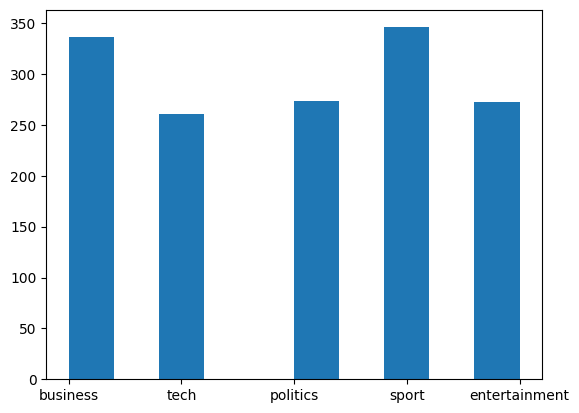
\includegraphics{./images/class_balanced.png} % Spécifiez le chemin de votre image
  \caption{Proportion des catégories d'article}
  \label{fig:classBalance}
\end{figure}

\subsection{Preprocessing}

Avant d'entamer l'implémentation de l'algorithme, il est essentiel de débuter par le prétraitement de notre jeu de données. Cette phase revêt une importance cruciale, car elle conditionnera la qualité de nos données et, par conséquent, celle de notre algorithme.\\

Il convient de souligner, dans un premier temps, que notre jeu de données est prêt à être traité. Les modèles de machine learning présentent des performances médiocres lorsqu'ils sont confrontés à des données textuelles. L'objectif principal est de surmonter cette contrainte en apportant des modifications subtiles à notre base de données.\\

Nous commencerons par éliminer la ponctuation des articles, car elle ne contribue pas à la valeur ajoutée de la classification. Dans cette démarche, nous recherchons le sens global plutôt que le sens par phrase. Toutefois, nous procéderons également à la suppression des mots dépourvus de sens sémantique, tels que les articles et les propositions. Voici un exemple des modifications apportées :\\

\textit{worldcom ex-boss launches defence lawyers defending former worldcom chief bernie ebbers against a battery of fraud charges have called a company whistleblower as their first witness. [..]}\\
\textit{worldcom exboss launches defence lawyers defending former worldcom chief bernie ebbers battery fraud charges called company whistleblower first witness cynthia [..]}\\

Enfin, toujours avec l'idée de nous intéresser seulement au sens global de l'article, nous allons réaliser une lemmatisation. Ce procédé nous permettra de mettre en évidence les mots clés des articles, normaliser le texte et améliorer la précision sémantique des modèles de machine learning.\\
Nous allons utiliser le lemmatizer \textit{WordNetLemmatizer}, entrainé sur la base de donnée \textit{WordNet}, pour lemmatiser notre jeu de donnée. Appliqué sur l'exemple précédent, nous obtenons le résultat suivant : \\

\textit{worldcom exboss launch defence lawyer defending former worldcom chief bernie ebbers battery fraud charge called company whistleblower first witness cynthia}

Enfin, on vectorisera les "nouveaux" articles afin d'obtenir un jeu de donnée vectoriels. Un type de donnée très largement utilisé pour le machine learning. Cette étape sera réalisé dans un pipeline qu'on présente dans la section suivante.

\section{Entrainement des modèles}

Afin de classifier les articles, nous allons tester des modèles de classification. Mais il nous reste avant celà une dernière étape : couper notre jeu de donnée en deux parties. La première sera utilisée pour l'entrainement et la seconde pour les testes. Il est habituellement recommendé, pour un jeu de donnée de notre envergure, de garder $77\%$ du data set pour l'entrainement et le reste pour le training. C'est ce qu'on appliquera ici.\\

\subsection{C-Support Vector Classification}.

Le premier modèle choisi est le Support Vector Classification. Ce modèle est généralement utilisé sur des data set de taille moyennes (~quelques milliers) mais il se trouve qu'il peut également être très performant sur de plus petits jeu de donnée de qualité.\\

\subsubsection{Pipeline}

Pour l'entrainement, on crée une pipeline permettant d'automatiser une séries de tâches. La pipeline se chargera ici de
\begin{itemize}
\item Vectoriser les articles grâce à la classe \texttt{CountVectorizer} fourni par \textit{Scikit-learn}
\item Tfid transforemr : j'ai oublié ce que ça fait
\item Entrainement du modèle SVC sur le jeu de donnée modifié.
\end{itemize}

\subsubsection{Validation}
















































\end{document}